% vim: set fenc=utf-8 ft=latex encoding=utf-8
% -*- mode: latex; coding: UTF-8; -*-

\newif\ifdraft
\drafttrue

\ifdraft
	\documentclass[conference, draftclsnofoot]{IEEEtran}
	\def\baselinestretch{1}
	\setlength{\marginparwidth}{2cm}
\else
	\documentclass[conferece, final]{IEEEtran}
\fi

\usepackage[T1]{fontenc}
\usepackage[utf8]{inputenc}

\newcommand{\TheTitle}{Visualizing Release Information of Linux}
\newcommand{\TheAuthors}{Evan Wilde}
\newcommand{\TheEmails}{etcwilde@uvic.ca}
\newcommand{\TheSubject}{Digesting large amounts of commit data}
\newcommand{\TheKeywords}{Linux, git, data structures, tree data structures}

\synctex=1

\usepackage[hyphens]{url}
\urlstyle{same}

\ifdraft
	\usepackage[unicode=true,bookmarks=false,breaklinks=false,
		pdfborder={0 0 0},backref=none,colorlinks=true]{hyperref}

\else
	\usepackage[unicode=true,bookmarks=false,breaklinks=false,
		pdfborder={0 0 0},backref=none,colorlinks=false]{hyperref}
\fi

\usepackage[nospace]{cite}

% Table Support
\usepackage{dcolumn}
\usepackage{longtable}

\usepackage{balance}
\usepackage{placeins}
\usepackage{multirow}

% Extra support
\usepackage{xspace}
\usepackage{caption}

% Fix any bad-hyphenations here
\hyphenation{}

% \ifdraft
%     \usepackage[colorinlistoftodos]{todonotes}
%     \newcommand{\evan}[1]{{\color{blue}\emph{Evan Says: #1}}\xspace}
%     \newcommand{\evantodo}[1]{{\color{blue}\emph{Evan Todo: #1}}\xspace}
%     \newcommand{\dmg}[1]{{\color{blue}\emph{dmg Says: #1}}\xspace}
%     \newcommand{\dmgtodo}[1]{{\color{blue}\emph{dmg Todo: #1}}\xspace}
% \else
%     \usepackage[disable]{todonotes}
%     \newcommand{\evan}[1]{}
%     \newcommand{\evantodo}[1]{}
%     \newcommand{\dmg}[1]{}
%     \newcommand{\dmgtodo}[1]{}
% \fi
    \usepackage[colorinlistoftodos]{todonotes}

\newcommand{\tool}{{\emph Linvis}\xspace}


    \newcommand{\evan}[1]{{\color{blue}\emph{Evan Says: #1}}\xspace}
    \newcommand{\evantodo}[1]{{\color{blue}\emph{Evan Todo: #1}}\xspace}
    \newcommand{\dmg}[1]{{\color{blue}\emph{dmg Says: #1}}\xspace}
    \newcommand{\dmgtodo}[1]{{\color{blue}\emph{dmg Todo: #1}}\xspace}


%%% Local Variables:
%%% mode: plain-tex
%%% TeX-master: t
%%% End:


\begin{document}

\title{\TheTitle}
\author{
\IEEEauthorblockA{\TheAuthors}
\IEEEauthorblockN{Department of Computer Science,
                    University of Victoria,
	    Canada.}
\IEEEauthorblockA{Email: \TheEmails}
}
\maketitle
\begin{abstract}

With an average of $x$ \evantodo{Fill in this number} merges into the Linux
kernel per release, containing thousands of commits, maintenance of older
versions of the kernel becomes nearly impossible. For security, performance,
and changing hardware, maintainers must understand the changes made to current
versions of the kernel, and how these changes fit into older versions in order
to merge them into the older versions. Current tools provide information about
the directed acyclic graph (DAG)\evan{Should I just replace this with DAG?}
which can be helpful for smaller projects, but with the scale and the number of
branches in the kernel, becomes overwhelming very quickly, if the tool doesn't
crash before generating the graph and handling the vast quantities information.

In this paper, I present a tool that uses the dataset collected by Daniel
German for \evantodo{Paper name\ldots} to generate a tool that can provide
better visualizations and better filtering.
\end{abstract}
\begin{IEEEkeywords}
\TheKeywords
\end{IEEEkeywords}

\section{Introduction}

Maintainers of older versions of the Linux kernel must sift through massive
number of commits with tools that are unable to filter and visualize the kernel
into a manageable size. Tools like gitk provide users with a full
view of the DAG (\ref{fig:DAG}), which for smaller projects can give a good
view of how the project is evolving. With larger, modular projects like the
Linux Kernel, the DAG becomes a tangled mess of lines that lose their meaning.
GitHub will also provide a DAG for most projects, but is unable to display it
for projects as large as the Linux Kernel (\ref{fig:github dag}).

\begin{figure}[h]
	\centering
	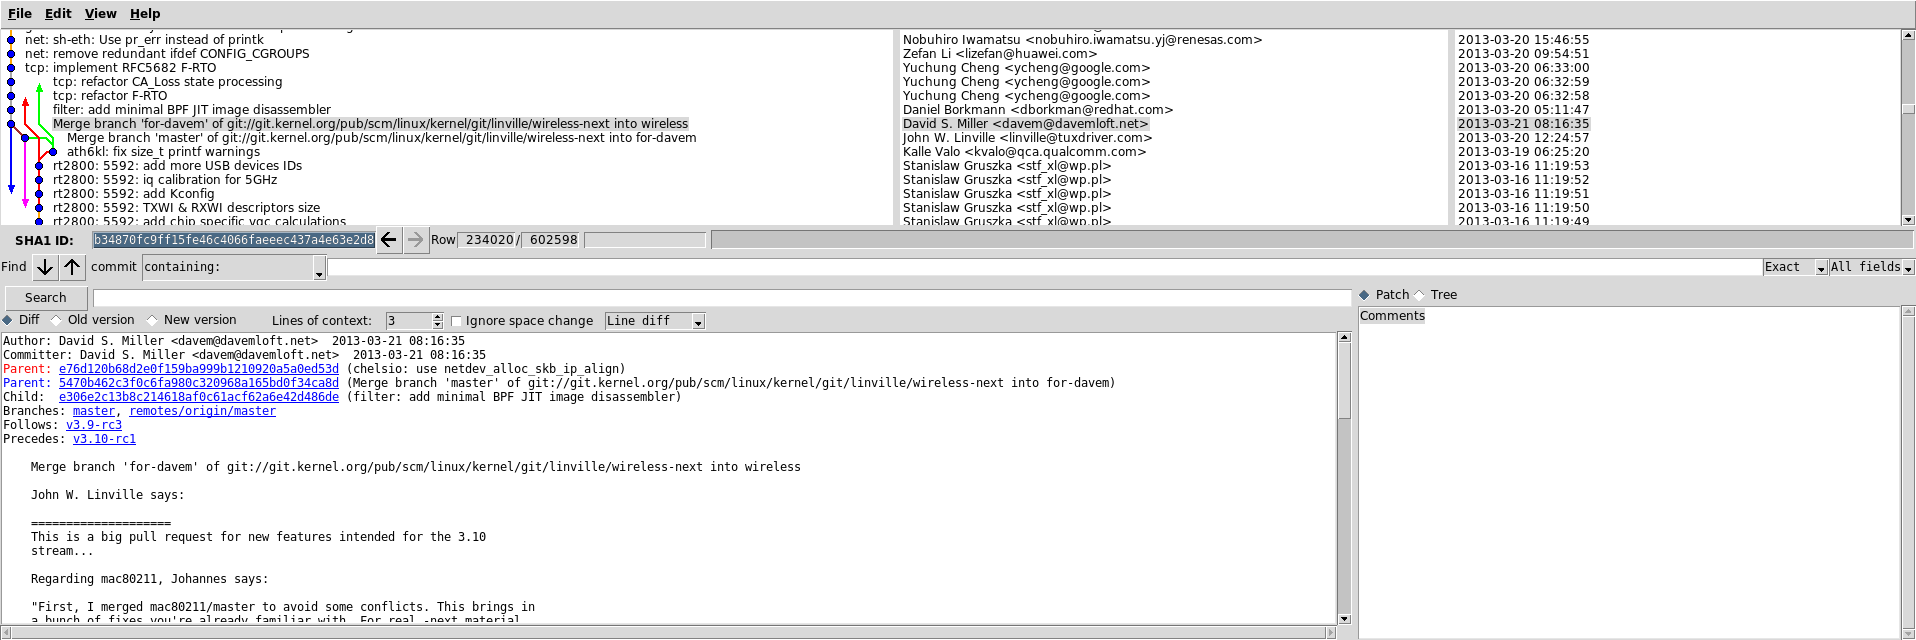
\includegraphics[height=1.5in]{figures/gitk.png}
	\caption{Portion of the Linux Kernel DAG}
	\label{fig:DAG}
\end{figure}

\begin{figure}[h]
	\centering
	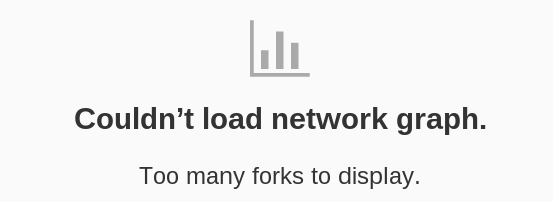
\includegraphics[height=1.5in]{figures/github_viewer.png}
	\caption{Github Error message}
	\label{fig:github dag}
\end{figure}


\section{Related Work}
Daniel German, et. al \evantodo{Find paper} recorded the Linux git repository
metadata from 2012 until 2015\evan{?}, storing information not available. They
also developed a heuristic to convert the DAG to a set of trees strung together
by the root as a linked list. We will call this structure a vine.

\evantodo{Make an picture of a vine with regards to the Linux kernel}

We built a web-based tool\footnote{\url{li.turingmachine.org}} to experiment
with the various ways to display and organize the release information of the
kernel.

%% The parts that make the tool usable
\section{Navigation}

Our system has multiple methods of allowing users to navigate through the data.

\subsection{Search}

Users search to filter out results they are not interested. We break the data
down by releases. From there, a user can further trim how many trees they want
to see by including a begin or end commit date, an author name, the commit id,
or keyword from a log preview to search for commits that match what they are
looking for.

\begin{figure}[h]
	\centering
	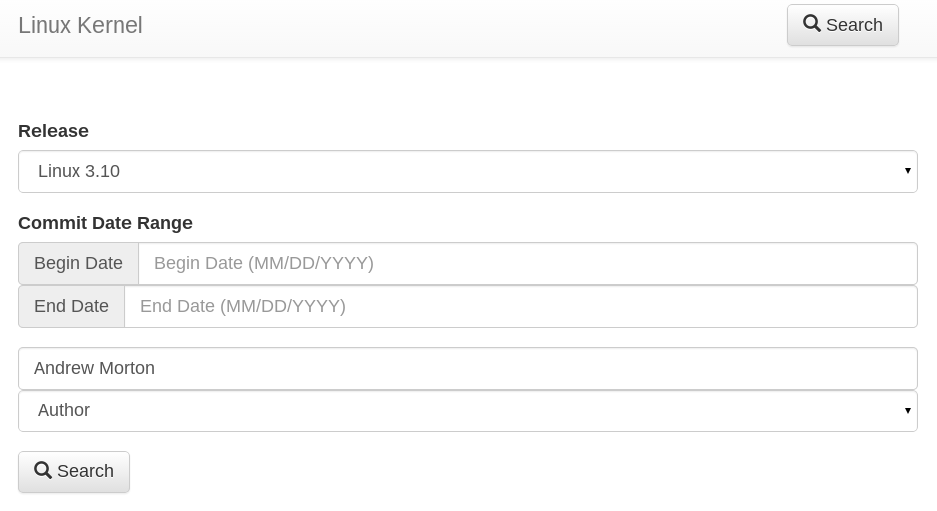
\includegraphics[height=1.5in]{figures/search_view.png}
	\caption{Search view}
	\label{fig:search_view}
\end{figure}

\begin{figure}[h]
	\centering
	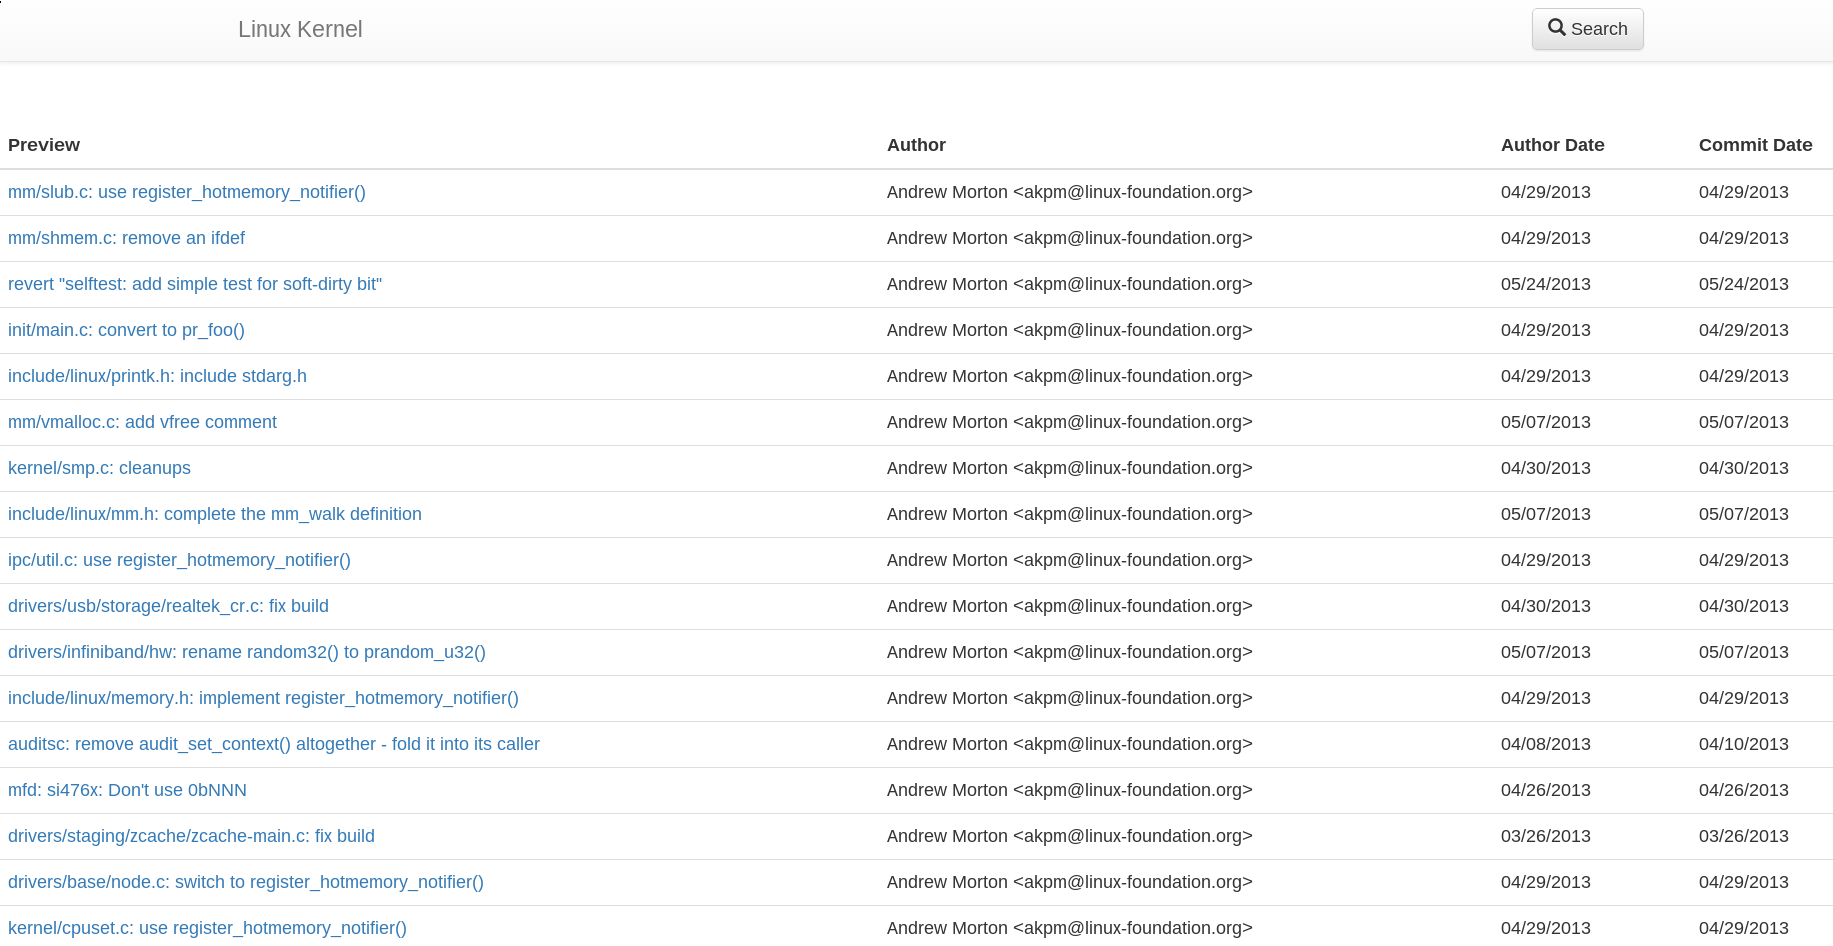
\includegraphics[height=1.5in]{figures/results_view.png}
	\caption{Results when searching for commits by Andrew Morton in Linux
	3.10}
	\label{fig:results_view}
\end{figure}


\subsection{Breadcrumbs}

\begin{figure}[h]
	\centering
	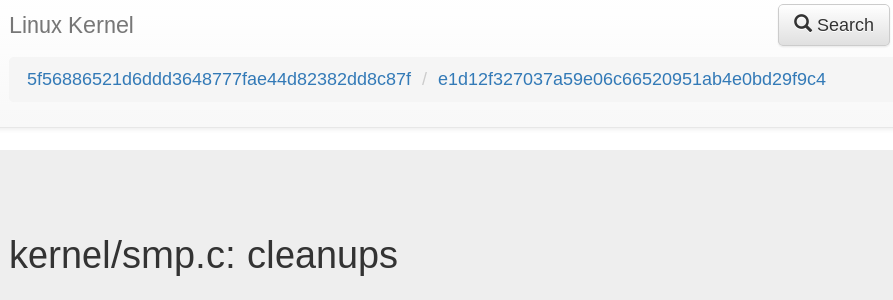
\includegraphics[height=1.0in]{figures/breadcrumbs.png}
	\caption{Generated Breadcrumbs}
	\label{fig:breadcrumbs}
\end{figure}

Our system provides breadcrumbs, allowing a user to move toward the root of the
tree and view the detailed view of the parent merge.

\section{Presentation}

\begin{figure}[h]
	\centering
	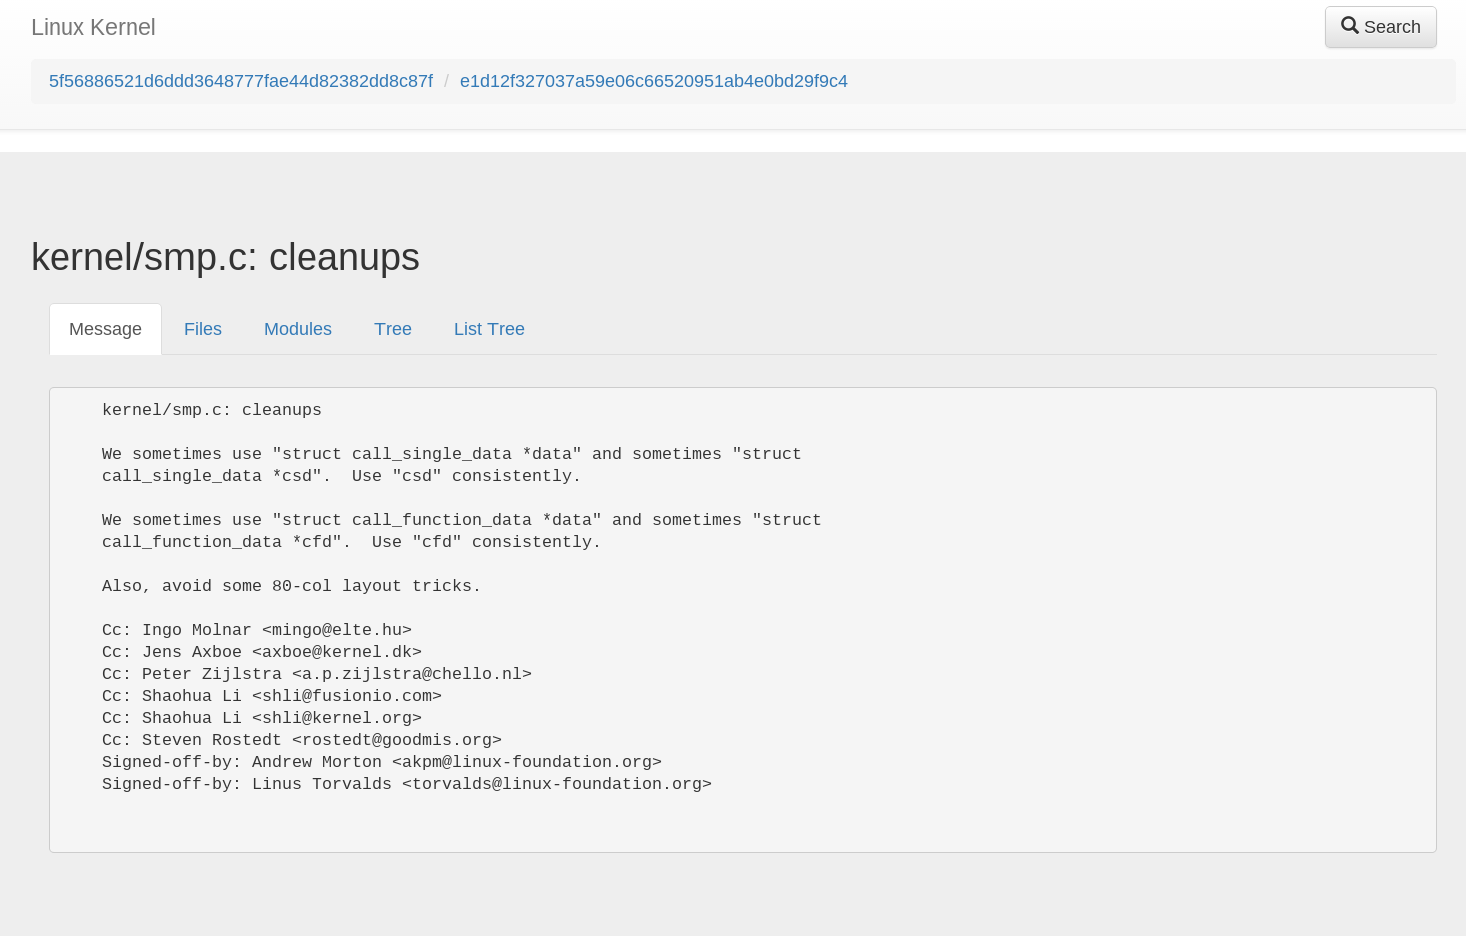
\includegraphics[height=1.5in]{figures/page.png}
	\caption{View of page}
	\label{fig:full page}
\end{figure}

We can provide information about what files were edited by a given commit or
merge. Due to the tree-structure of the data, we can perform a tree traversal
to determine the number of files and modules touched within the merges.



%% The special parts that make the tool special
\section{Date Range Queries}

Git does not store the date that a given commit is merged into another branch,
it stores the date that the commit was authored. This is why the data collected
by Daniel German becomes important. His recording system monitored each commit
as it moved through the kernel, storing the commit and author dates of each
commit.

A commit may be created and not be merged with the kernel until much later. It
is these merges that make performing date range queries using the conventional
tools useless as they will not be included even though they are having an
effect on the kernel in the requested date range. Our system splits the kernel
into releases, and only looks at the dates of the merges performed by Linus
directly into the master branch. From there, we are able to construct the trees
below each of these merges, which may contain commits from before the begin
date of the selected range, or after the end date for the given range. This
provides information about the commits that come from older branches that were
pulled forward, or patches that were merged backward into an older version of
the kernel as part of maintenance.


\section{Visualization}

Recognizing each merge with the master branch of the kernel as a subtree helps
remove information that is unnecessarily shown in other tools, like the DAG.
There are many ways of visualizing trees, including a standard tree
visualization(\ref{fig:moderate_tree_view}). An issue with a standard tree visualization
is that it can only display a certain amount of information at each node before
it becomes cluttered and incomprehensible, furthermore, as we can see in figure 
(\ref{fig:large_tree_view}), if there are many nodes, even limited information
becomes cluttered.

\evantodo{Make the lines and nodes bigger and brighter in the tree screenshots}
\begin{figure}[h]
	\centering
	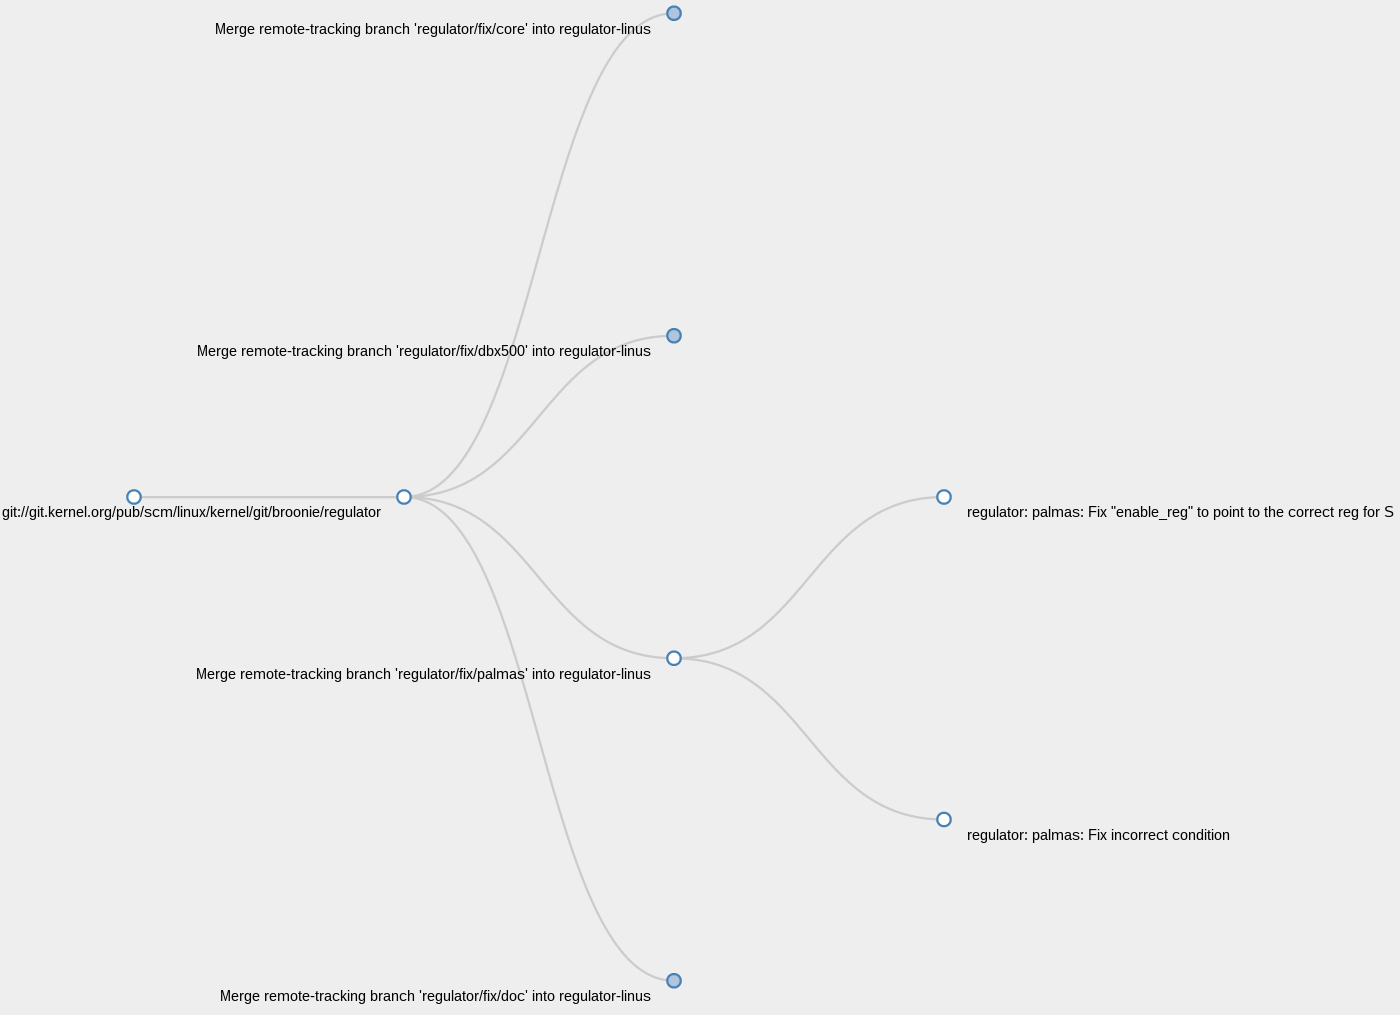
\includegraphics[height=1.5in]{figures/tree_viewer.png}
	\caption{Moderately sized tree view tree}
	\label{fig:moderate_tree_view}
	% CID: 042dd60ca6dec9a02cefa8edd67de386e35755d6
\end{figure}

\begin{figure}[h]
	\centering
	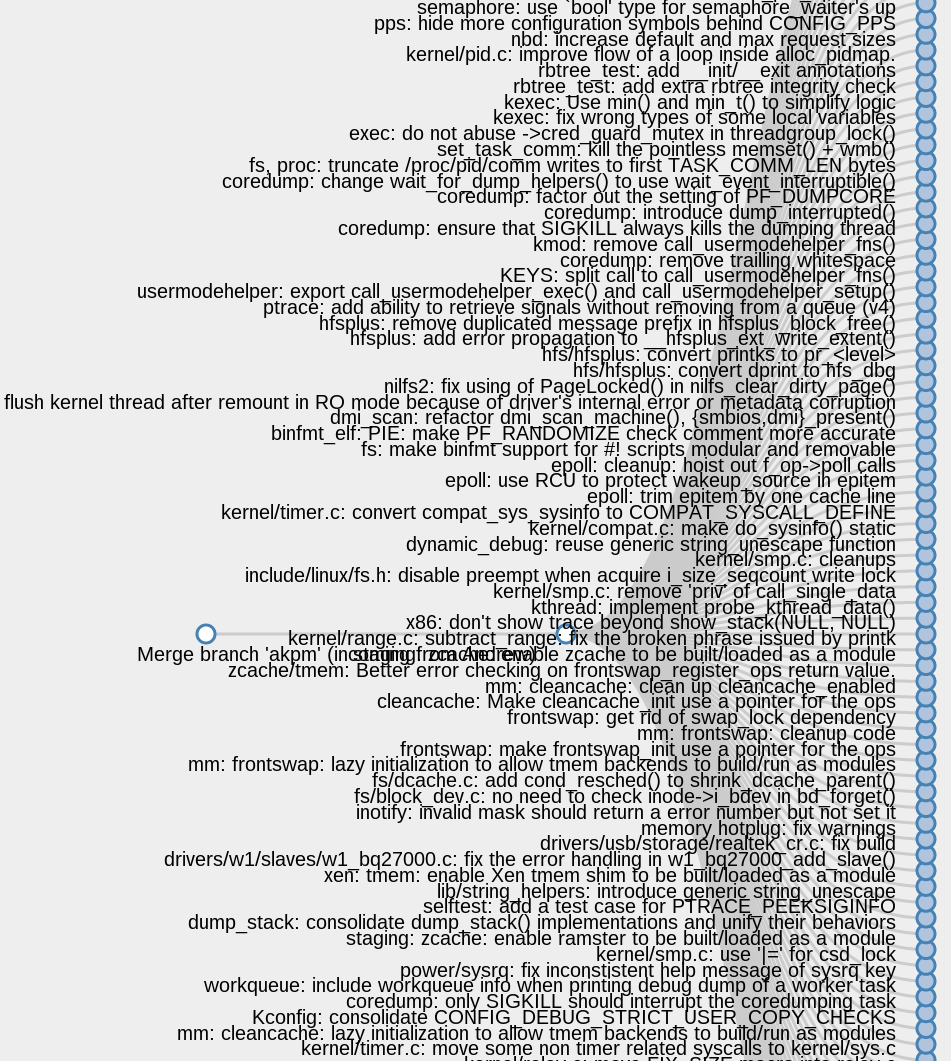
\includegraphics[height=2.5in]{figures/tree_viewer_large.png}
	\caption{Large tree view tree}
	\label{fig:large_tree_view}
	% CID : 5f56886521d6ddd3648777fae44d82382dd8c87f
\end{figure}

Perhaps a more useful tree is the list-tree, which allows us to show the
layers in the tree using indentation. This also allows us to create click-able
links to the corresponding items in the tree.

\begin{figure}[h]
	\centering
	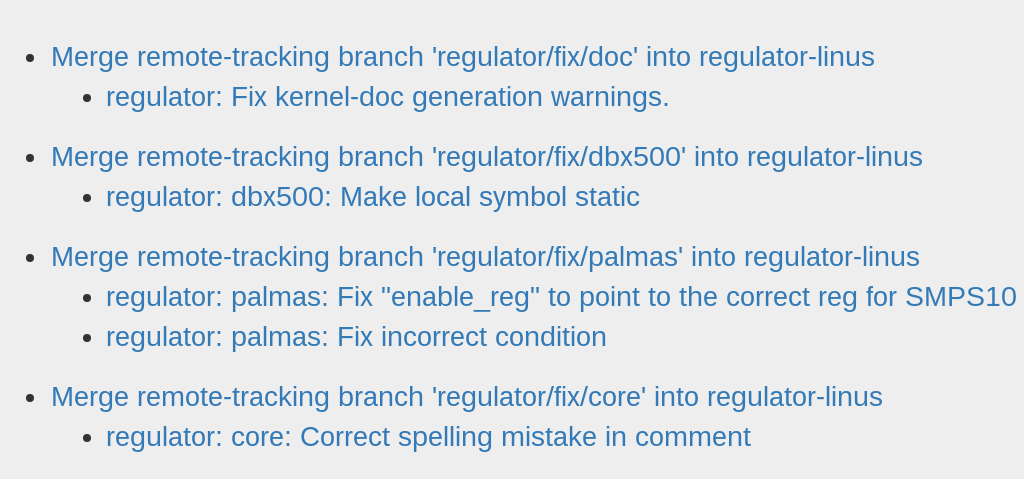
\includegraphics[height=1.5in]{figures/list_viewer.png}
	\caption{Moderately sized list view tree}
	\label{fig:moderate_list_view}
	% CID: 042dd60ca6dec9a02cefa8edd67de386e35755d6
\end{figure}

\begin{figure}[h]
	\centering
	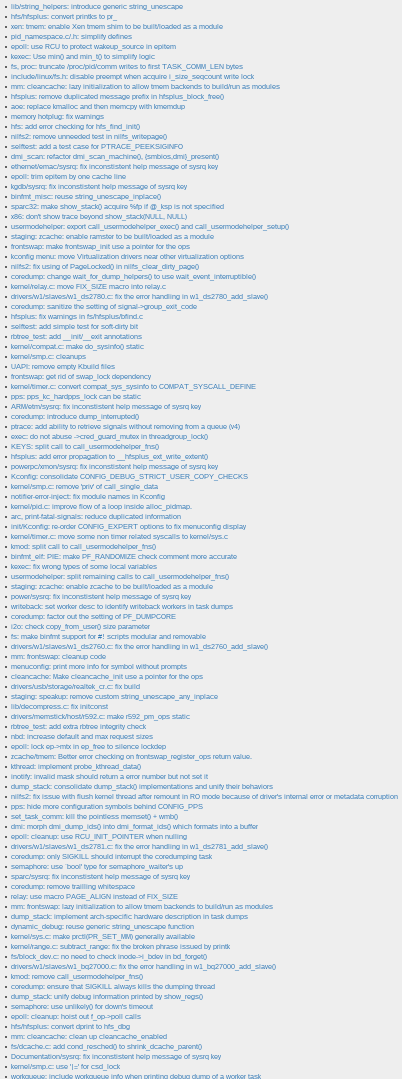
\includegraphics[height=3.5in]{figures/list_viewer_large.png}
	\caption{Large list view tree}
	\label{fig:large_list_view}
	% CID : 5f56886521d6ddd3648777fae44d82382dd8c87f
\end{figure}


Figures \ref{fig:moderate_tree_view} and \ref{fig:moderate_list_view} display
the same subtree, however, the list-based subtree provides a cleaner, faster
way to navigate the tree, whereas the graphical tree view provides a way to
hide unnecessary branches of the tree.

We can see in figures \ref{fig:large_tree_view} and \ref{fig:large_list_view}
that neither representation of the trees can cope with the larger trees in a
clean manner. These larger trees are, however, and exception to the rule. These
trees are from one of the many memory management patches by Andrew Morton,
which get the name ``Andrews patch bombs''. Andrews patches are very wide trees
that have only leaves and no internal merging. Conversely, the networking
modules are far larger with massive breadth and some depth. Overall the Linux
kernel has a very flat structure wit little depth, the deepest node being $5$
merges away \evantodo{verify this} from the root merge into the kernel.


\evantodo{Build sunburst tree into visualizer, then add pictures}

\end{document}

